\documentclass[a4paper,12pt,oneside]{article}

\usepackage[textwidth=400pt,textheight=730pt,top=60pt,left=100pt]{geometry}
\usepackage[english]{babel}
\usepackage{hyperref}
\usepackage[nolist]{acronym}
%\usepackage[onehalfspacing]{setspace}
\usepackage{setspace}
\usepackage{booktabs}
\usepackage{graphicx}
\usepackage{float}
\usepackage{amsmath}
\usepackage{listings}
\usepackage{cite}
\usepackage{tikz}
\usepackage{wasysym}
\usepackage{amssymb}
\usepackage{dirtree}
\usepackage[figuresright]{rotating}
\usepackage{subcaption}
\usepackage{adjustbox}
\usepackage{lineno}
\usepackage{multicol}
\linenumbers

\usetikzlibrary{matrix,calc}
%---------------------------
%\usepackage{showframe}
%
\def\Tab{\mathcal{T}^\text{thrown}}
\def\WeightGridTrials{w^\text{grid-trials}}
\def\WeightGridSuccesses{w^\text{grid-intense}}
%
\begin{document}
%
\noindent
%
\LARGE
\textbf{Cutting events to estimate\\instrument-response-functions}
\normalsize\\
%
\begin{center}
Sebastian Achim Mueller, 2020\,March\,25
\end{center}
%
The detection of gamma-ray-sources with the on-off-measurement, and being able to trigger with established technology \cite{delagnes2006sam} are important aspects of an instrument's performance.\\
%
In our simulation, we represent these different aspects with two weights $f_j^\text{thrown}$, and $f_j^\text{detected}$ which we assign to each $j$-th thrown air-shower.
%
Table \ref{TabAspects} shows the cuts relevant for $f_j^\text{thrown}$, and $f_j^\text{detected}$.
%
Section \ref{SecEffectiveQuantity} shows how these wights for thrown and detected air-showers contribute to the effective area, and acceptance.
%
Section \ref{SecCuts} lists the cuts, and Section \ref{SecOnOffMeasurement} traces the weights through the on/off-measurement from the $j$-th air-shower to the final signal- and background-rates.
%
\def\True{0\,or\,1}
%
\begin{table}[H]
\resizebox{\textwidth}{!}
{%
\begin{tabular}{ll|rrrr|rrrr}
 & & \multicolumn{4}{c}{trigger} & \multicolumn{4}{c}{on/off}\\
 %
 & & \multicolumn{2}{c}{gamma-ray} & \multicolumn{2}{c}{cosmic-ray} & \multicolumn{2}{c}{gamma-ray} & \multicolumn{2}{c}{cosmic-ray}\\
%
&%
&%
\multicolumn{2}{c}{area} &%
\multicolumn{2}{c}{acceptance} &%
\multicolumn{2}{c}{area} &%
\multicolumn{2}{c}{acceptance}\\
%
&%
&%
\multicolumn{2}{c}{$A_\text{gamma}^\text{trigger}(E)$} &%
\multicolumn{2}{c}{$\aleph_p^\text{trigger}(E)$} &%
\multicolumn{2}{c}{$A_\text{gamma}^\text{on/off}(E)$} &%
\multicolumn{2}{c}{$\aleph_p^\text{on/off}(E)$}\\
%
&%
&%
$f_j^\text{thrown}$&%
$f_j^\text{detected}$&%
$f_j^\text{thrown}$&%
$f_j^\text{detected}$&%
$f_j^\text{thrown}$&%
$f_j^\text{detected}$&%
$f_j^\text{thrown}$&%
$f_j^\text{detected}$\\
%
\noalign{\smallskip}\hline\noalign{\smallskip}
%
\ref{SecPassedTrigger} &%
Passed trigger &%
- &%
\True &%
- &
\True &%
- &%
\True &%
- &%
\True\\
%
\ref{SecPassedCherenkovcleaning} &%
Passed Cherenkov-cleaning &%
- &%
- &%
- &%
- &%
- &%
\True &%
- &%
\True\\
%
\ref{SecPassedFeatureExtraction} & %
Passed feature-extraction&%
- &%
- &%
- &%
- &%
- &%
\True &%
- &%
\True\\
%
\ref{SecReconstructedToBeAGammaRay} &%
\vtop{%
\hbox{\strut $\gamma_\text{reco} \geq \gamma_\text{threshold}$}%
\hbox{\strut \hspace{0.5cm}Reconstructed to}%
\hbox{\strut \hspace{0.5cm}be a gamma-ray}}&%
- &%
- &%
- &%
- &%
- &%
\True &%
- &%
\True\\
%
\ref{SecTrueDirectionInPotentialOnOffRegion} &%
\vtop{%
\hbox{\strut $\angle(\Theta_\text{plenocope},\Theta_\text{true}) \leq \delta_\text{potential-on/off}$}%
\hbox{\strut \hspace{0.5cm}True direction in}%
\hbox{\strut \hspace{0.5cm}potential on/off-region}}&%
\True &%
\True &%
- &%
- &%
\True &%
\True &%
- &%
-\\
%
\ref{SecReconstructedDirectionInOnRegion} &%
\vtop{%
\hbox{$\angle(\Theta_\text{true},\Theta_\text{reco}) \leq \delta_\text{on/off}(E_\text{reco})$}%
\hbox{\strut \hspace{0.5cm}Reconstructed}%
\hbox{\strut \hspace{0.5cm}direction in}%
\hbox{\strut \hspace{0.5cm}on-region}}&%
- &%
- &%
- &%
- &%
- &%
\True &%
- &%
-\\
%
\ref{SecReconstructedDirectionInFieldOfView} &%
\vtop{%
\hbox{$\angle(\Theta_\text{plenocope},\Theta_\text{reco}) \leq \delta_\text{fov}$}%
\hbox{\strut \hspace{0.5cm}Reconstructed}%
\hbox{\strut \hspace{0.5cm}direction in}%
\hbox{\strut \hspace{0.5cm}field-of-view}}&%
- &%
- &%
- &%
- &%
- &%
- &%
- &%
\True\\
%
\ref{SecProbabilityToBeOnRegion} &%
\vtop{%
\hbox{\strut Probability to be}%
\hbox{\strut \hspace{0.5cm}in on-region}}&%
- &%
- &%
- &%
- &%
- &%
- &%
- &%
$\frac{\Omega_\text{on/off}(E_\text{reco})}{\Omega_\text{fov}}$ \\
%
\noalign{\smallskip}\hline
\end{tabular}
%
}% resizebox
%
\caption{%
The cuts for triggering, and on/off-measurement.
%
The relevant weights in a column are multiplied to estimate $f_j^\text{thrown}$, and $f_j^\text{detected}$.
%
Cuts with dashes '-' are not relevant.
%
Table \ref{TabVariables}, and Figure \ref{FigFieldOfView} explain the variables.
%
}
\label{TabAspects}
\end{table}
%
%
\begin{table}[H]
\begin{tabular}{ll}
\hline\noalign{\smallskip}
$A$ & effective area\\
$\aleph$ & effective acceptance, (area$\times$solid angle)\\
$\Theta_\text{true}$ & True direction of particle\\
$\Theta_\text{reco}$ & Reconstructed direction of particle\\
$\Theta_\text{plenocope}$ & Pointing direction of plenoscope\\
$\angle(\Theta_\text{a}, \Theta_\text{b})$ & Angle between directions $\Theta_\text{a}$, and $\Theta_\text{b}$\\
$E$ & True energy of particle\\
$E_\text{reco}$ & Reconstructed energy of particle\\
$\gamma_\text{reco}$ & Reconstructed probability to be a gamma-ray \\
$\gamma_\text{threshold}$ & Recognized as gamma-ray when $\gamma_\text{reco} \geq \gamma_\text{threshold}$\\
$\sigma_\text{on/off} = 68\%$ & Fraction of true gamma-rays with $\Theta_\text{reco}$ in the on-region.\\
$\delta_\text{on/off}(E_\text{reco})$ & Angular radius for on-, off-regions, e.g. 0.8$^\circ$ at 1\,GeV.\\
 & \hspace{0.5cm}Radius contains $\sigma_\text{on/off}$ of the true gamma-rays $\Theta_\text{reco}$.\\
$\Omega_\text{on/off}(E_\text{reco})$ & Solid angle of the on-region\\
$\delta_\text{fov}$ & Angular radius of plenoscope's field-of-view, 3.25$^\circ$\\
$\Omega_\text{fov}$ & Solid angle of plenoscope's field-of-view\\
$E_\text{threshold}$ & Energy-threshold of plenoscope $\approx 1\,$GeV\\
$\delta_\text{potential-on/off}$ & Angular radius , e.g. $\delta_\text{fov} - \delta_\text{on/off}(E_\text{threshold}) \approx 2.5^\circ$\\
\noalign{\smallskip}\hline
\end{tabular}
\caption{Variables, see also Figure \ref{FigFieldOfView}.}
\label{TabVariables}
\end{table}
%
%
\begin{figure}
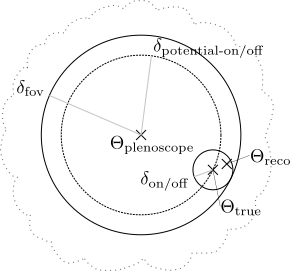
\includegraphics[width=0.76\textwidth]{field_of_view.png}
\caption{
Sky-dome with plenoscope's field-of-view.
%
Here a suspected source of gamma-rays at $\Theta_\text{true}$ happens to be on the edge of potential on/off-regions.
%
This is the largest angle possible between $\Theta_\text{true}$ and $\Theta_\text{plenoscope}$.
%
Dotted cloud marks the pool of all thrown particle directions.
%
Not to scale.
%
}
\label{FigFieldOfView}
\end{figure}
%
\section{Cuts}
\label{SecCuts}
%
\subsection{Passed trigger}
\label{SecPassedTrigger}
%
The thrown air-shower creates a light-field-sequence dense enough to trigger the readout in the plenoscope's light-field-sensor.
%
The light-field-sequence is copied to permanent storage.
%
A plenoscope-event is created.
%
There is potential dead time in which the plenoscope is blind.
%
\subsection{Passed Cherenkov-cleaning}
\label{SecPassedCherenkovcleaning}
%
We are able to classify Cherenkov-photons based on their density in a plenoscope-event.
%
\subsection{Passed feature-extraction}
\label{SecPassedFeatureExtraction}
%
We are able to extract features from a plenoscope-event.
%
\subsection{Reconstructed to be a gamma-ray}
\label{SecReconstructedToBeAGammaRay}
%
Our gamma-hadron-separation estimates the air-shower's probability to be induced by a gamma-ray
%
\begin{eqnarray*}
\gamma_\text{reco} \geq \gamma_\text{threshold}
\end{eqnarray*}
%
to be above a predefined threshold.
%
\subsection{True direction in potential on/off-region}
\label{SecTrueDirectionInPotentialOnOffRegion}
%
The angle between the primary particle's true direction $\Theta_\text{true}$, and the plenoscope's pointing $\Theta_\text{plenocope}$ is contained in the radius to put the centers of potential on/off-regions
%
\begin{eqnarray*}
\angle(\Theta_\text{plenocope},\Theta_\text{true}) \leq \delta_\text{potential-on/off}.
\end{eqnarray*}
%
This ensures that our suspected source to be detected in an on/off measurement is not on the edge of the plenoscope's field-of-view, but in a solid angle which allows the on-region to be fully contained in the plenoscope's field-of-view.
%
\subsection{Reconstructed direction in on-region}
\label{SecReconstructedDirectionInOnRegion}
%
The reconstructed direction $\Theta_\text{reco}$ of a true gamma-ray must be contained in the on-region of the suspected source at direction $\Theta_\text{true}$
%
\begin{eqnarray*}
\angle(\Theta_\text{true},\Theta_\text{reco}) \leq \delta_\text{on/off}(E_\text{reco}).
\end{eqnarray*}
%
This is the signal in the on/off-measurement.
%
\subsection{Reconstructed direction in field-of-view}
\label{SecReconstructedDirectionInFieldOfView}
%
Cosmic-rays which are mistaken for gamma-rays must only be taken into account when their reconstructed direction is in the plenoscope's field-of-view, because we also only take into account true gamma-rays when their reconstructed direction is in the plenoscope's field-of-view.
%
\begin{eqnarray*}
\angle(\Theta_\text{plenoscope},\Theta_\text{reco}) \leq \delta_\text{fov}
\end{eqnarray*}
%
For gamma-rays, where we can relate to the true direction, this cut is implicitly done in cut number \ref{SecReconstructedDirectionInOnRegion}.
%
\subsection{Probability to be in on-region}
\label{SecProbabilityToBeOnRegion}
%
This is not a binary cut, but a floating weight.
%
True cosmic-rays which are reconstructed to be gamma-rays are assigned a weight
%
\begin{eqnarray*}
\frac{\Omega_\text{on/off}(E_\text{reco})}{\Omega_\text{fov}}.
\end{eqnarray*}
%
For a weight $1.0$, the cosmic-ray's air-shower, which is mistaken for a gamma-ray, will contribute fully to the acceptance of cosmic-rays $\aleph^\text{on/off}_p$, regardless of its reconstructed direction $\Theta_\text{reco}$.
%
But what we actually want is the air-shower to only contribute when it was reconstructed to be within the on-region of our suspected source of gamma-rays.
%
Therefore, we reduce the weight of the air-shower by the ratio of solid angles for the on-region, and the field-of-view.
%
\section{The on/off-measurement}
\label{SecOnOffMeasurement}
%
For the on-off-measurement \cite{li1983analysis}, our simulation estimates the expected signal-rate
%
\begin{eqnarray}
N_s &=& \sigma_\text{on/off} \int F_\text{gamma}(E)\,A_\text{gamma}^\text{on/off}(E) \mathrm{d}E
\label{EqSignalRate}
\end{eqnarray}
%
in the on-region surrounding a suspected source of gamma-rays.
%
Here $\sigma_\text{on/off}$ takes into account, that only a fraction $\sigma_\text{on/off} = 68\%$ of true gamma-rays is reconstructed to be in the on-region.
%
Correspondingly, our simulation estimates the background-rate
%
\begin{eqnarray*}
{N_\text{off}}_p &=& \int \Phi_p(E)\,\aleph_p^\text{on/off}(E) \mathrm{d}E
\end{eqnarray*}
%
in the corresponding off-region induced by cosmic-ray $p$.
%
The total rate of background
%
\begin{eqnarray*}
N_\text{off} &=& \sum_{p = [\text{e}^-, \text{e}^+, \text{p}^-, \text{He}, \dots]} {N_\text{off}}_p
\end{eqnarray*}
%
is the sum of background rates caused by all relevant cosmic-rays.
%
We take the differential flux of a point-source
%
\begin{eqnarray*}
F_\text{gamma}(E) &/& \mathrm{m}^{-2}\,\mathrm{(GeV)}^{-1}\,\mathrm{s}^{-1}
\end{eqnarray*}
%
from e.g. Fermi-LAT's catalog \cite{acero2015fermi3fgl}, and we use measurements of e.g. \mbox{AMS-02} \cite{aguilar2015precision, aguilar2014precision} for the differential flux of the diffuse cosmic-rays
%
\begin{eqnarray*}
\Phi(E)_p &/& \mathrm{m}^{-2}\,\mathrm{sr}^{-1}\,\mathrm{(GeV)}^{-1}\,\mathrm{s}^{-1}.
\end{eqnarray*}
%
Our simulation has to estimate the effective area for gamma-rays
%
\begin{eqnarray*}
A_\text{gamma}^\text{on/off}(E) &/& \text{m}^2
\end{eqnarray*}
%
and the effective acceptances for cosmic-rays
%
\begin{eqnarray*}
\aleph_p^\text{on/off}(E) &/& \text{m}^2\,\text{sr}.
\end{eqnarray*}
%
To estimate $A_\text{gamma}^\text{on/off}(E)$, and $\aleph_p^\text{on/off}(E)$, we use Equation \ref{EqEffectiveQuantity} and assign the weights $f_j^\text{thrown}$, and $f_j^\text{detected}$ to each $j$-th thrown air-shower according to \mbox{Table \ref{TabAspects}}.
%
\section{Effective area and acceptance}
\label{SecEffectiveQuantity}
%
For energy-bin $e$, the effective quantity $Q^\text{effective}_e$, this is either area $A_e$ or acceptance $\aleph_e$, is
%
\begin{eqnarray}
Q^\text{effective}_e &=& \frac{Q^\text{detected}_e}{C^\text{thrown}_e},
\label{EqEffectiveQuantity}
\end{eqnarray}
%
with
\begin{eqnarray*}
Q^\text{detected}_e &=& \sum_{j=0}^J\,m^e_j\,f^\text{detected}_j\,\WeightGridSuccesses_j\,Q^\text{max}_j,
\end{eqnarray*}
%
and
%
\begin{eqnarray*}
C^\text{thrown}_e &=& \sum_{j=0}^J\,m^e_j\,f^\text{thrown}_j\,\WeightGridTrials_j.
\end{eqnarray*}
%
where $Q^\text{max}_j$ is the maximum scatter of the quantity, this is either $A^\text{max}_j$ or $\aleph^\text{max}_j$.
%
The weights $\WeightGridSuccesses_j$, and $\WeightGridTrials_j$ are related to our grid.
%
And the weight $m^e_j$ is 1 when the $j$-th air-shower is in the $e$-th energy-bin, and 0 otherwise.
%
%
\bibliographystyle{apalike}
\bibliography{references.bib}   % name your BibTeX data base
\end{document}
%